\section{The Proposed Solution}
\label{sec:solution}

\subsection{Overall Architecture}

The Moroccan Legal RAG system follows a layered architecture organized around
two main flows: the ingestion flow (PDF $\rightarrow$ vector knowledge base)
and the inference flow (question $\rightarrow$ generated answer). Each layer
is independently interchangeable.

\subsection{Ingestion-Pipeline Components}

\subsubsection{PDF Classification and Extraction with VLM Correction}

A PDF classifier determines whether a document is digital (extractable text)
or scanned (image-based). For scanned PDFs, the pipeline comprises: (1)
PyMuPDF renders each page as a PNG image, (2) EasyOCR performs Arabic text
recognition on GPU, (3) Gemma 4 in vision mode corrects OCR errors with a
specialized prompt, following the post-OCR correction paradigm of
\cite{benajiba2023arabic}, and (4) post-processing corrects the Arabic
visual order.

\subsubsection{Legal Text Cleaning}

The \texttt{LegalTextCleaner} removes noise specific to Moroccan legal
documents: repeated headers/footers, page numbers, watermarks, table-of-
contents artifacts, duplicate paragraphs, incorrect line breaks, and
non-text artifacts.

\subsubsection{Arabic Normalization}

The \texttt{ArabicNormalizer} applies standardized Arabic preprocessing:
Unicode NFKC normalization, alef unification, diacritic removal, tatweel
(kashida) removal, digit normalization, and punctuation spacing.

\subsubsection{Structural Parsing}

The \texttt{LegalStructureParser} extracts the hierarchical structure:
books/parts, chapters, sections, and articles matching the pattern
``Article $X$'' (\emph{al-madda $X$}). Each article is enriched with complete
hierarchical context (law name, number, book, chapter, section) and
serialized to JSON.

\subsubsection{Vector Ingestion}

Articles are contextualized with a prefix (e.g., ``[Penal Code] [Section 3]
Article 147: \ldots''), embedded via BGE-M3 (1024d), and inserted into
PostgreSQL with an HNSW index ($m=16$, ef\_construction $=200$).

\subsection{Inference-Pipeline Components}

\subsubsection{REST API (FastAPI)}

The REST API is built with FastAPI~\cite{fastapi2023}. Six endpoints are
exposed under \texttt{/api/v1}: health check, pure search, full Q\&A (RAG),
laws listing, PDF upload, and conversation history.

\subsubsection{Hybrid Search Engine}

Three interchangeable strategies are implemented via the Strategy pattern.

\textbf{Dense retrieval.} The query is encoded into a 1024-dimensional vector
and searched via pgvector's cosine-distance operator $\mathtt{<=>}$.

\textbf{BM25 retrieval.} PostgreSQL FTS with the Arabic dictionary was
abandoned due to poor performance. An in-memory \texttt{BM25Okapi} index was
implemented with a specialized Arabic tokenizer: (1) normalization via
\texttt{ArabicNormalizer}, (2) Unicode regex word extraction, (3) removal of
60+ legal stop-words, (4) filtering of short tokens ($<2$ characters). This
approach achieves Recall@5 of 41.67\% and Hit@5 of 46.88\%.

\textbf{Reciprocal Rank Fusion.} Top-$N$ results from each strategy ($N=20$)
are fused using:
\begin{equation}
  \label{eq:rrf}
  \mathrm{RRF}(d) = \sum_{s \in \{\mathrm{dense}, \mathrm{bm25}\}}
  \frac{1}{k + r_s(d)},
\end{equation}
where $k = 60$ is the fusion constant and $r_s(d)$ is the rank of document
$d$ in strategy $s$. Figure~\ref{fig:rrf} illustrates the fusion procedure.

\begin{figure}[t]
  \centering
  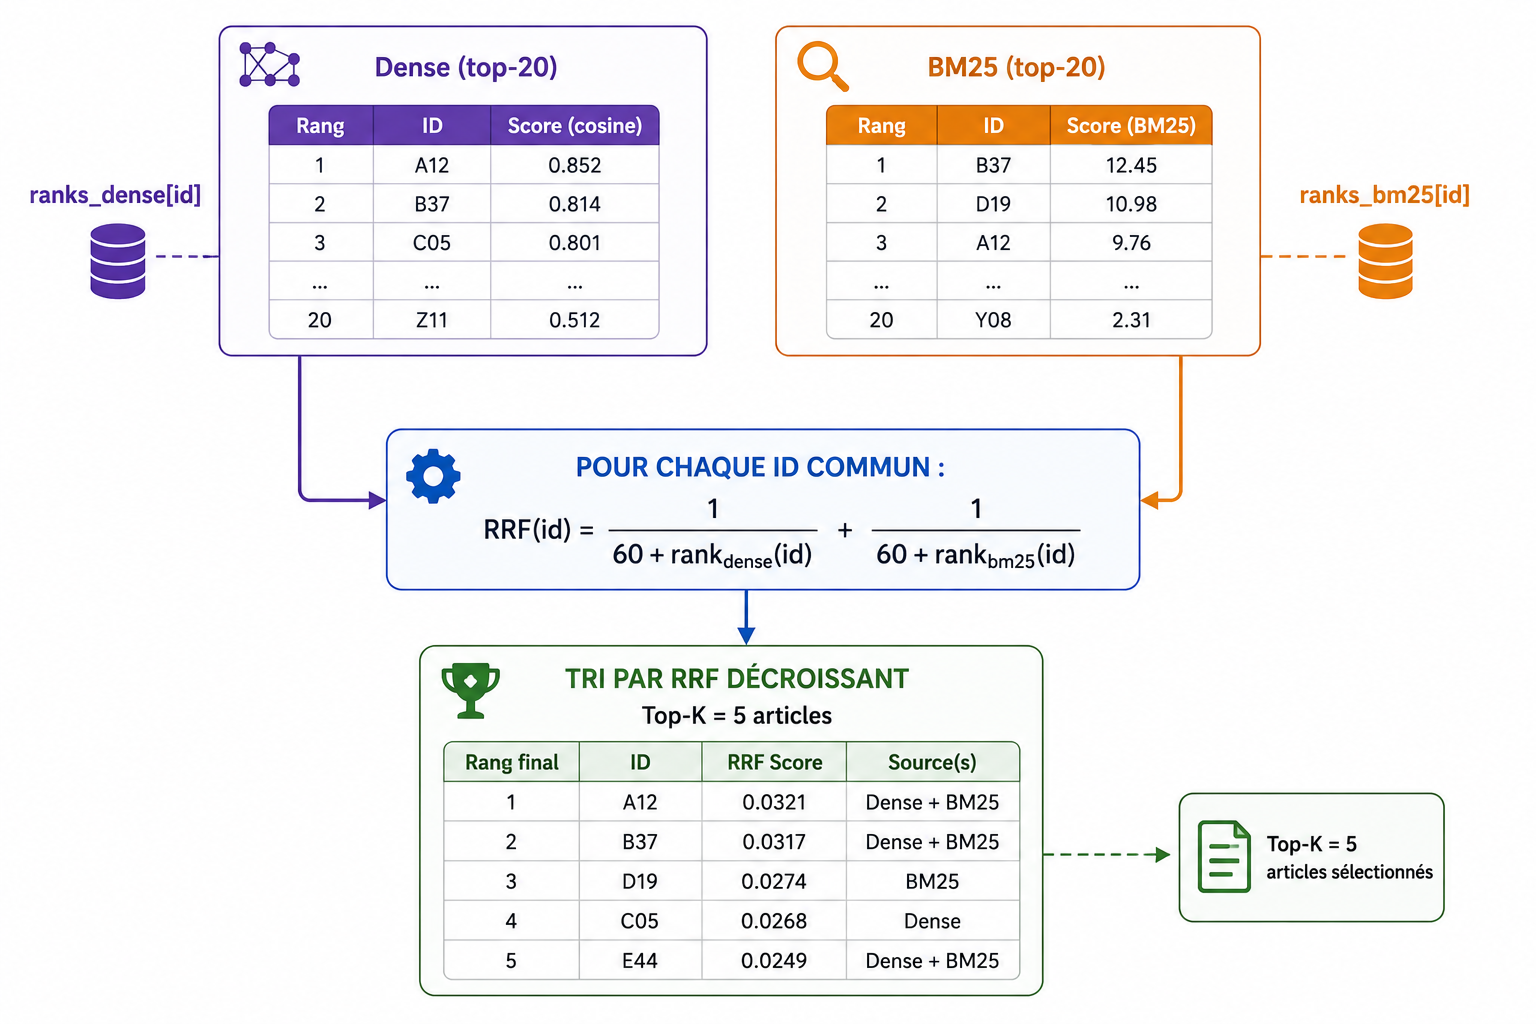
\includegraphics[width=0.92\columnwidth]{images/rrf_fusion.png}
  \caption{Reciprocal Rank Fusion: dense (top-20) and BM25 (top-20) rankings
           are combined with the RRF formula and sorted to produce the final
           top-$K$ list.}
  \label{fig:rrf}
\end{figure}

\subsubsection{LLM Generation Module}

The generation module builds a structured prompt from retrieved articles and
calls a remote LLM. The prompt includes: (1) retrieved legal texts numbered
and sourced, (2) a system instruction specifying the Moroccan legal-assistant
role, the grounding rule, and the output format, (3) the user's question. The
LLM is Gemma 4 2B, quantized to Q4\_K\_XL and served via llama.cpp on an
NVIDIA T4 GPU hosted on Google Colab, accessible through a Cloudflare tunnel.
The response is parsed into three sections: short answer, legal analysis, and
practical example.

\subsection{Data Infrastructure}

PostgreSQL 16 with pgvector 0.7.4~\cite{pgvector2023} stores
\texttt{legal\_chunks} (articles with 1024d embeddings, domain metadata,
HNSW index) and \texttt{conversations} (session history with JSONB sources).

\subsection{User Interface}

The web interface is developed with SvelteKit 5~\cite{sveltekit2024} and
Tailwind CSS 4, with full Arabic (RTL) support, offering a search page,
results page with structured answers, law explorer with hierarchical tree,
conversation history, PDF upload interface, and system health dashboard.
